\chapter{An Autonomous Robotic Team for the Rapid Characterization of Novel Environments}

In this chapter, we present preliminary results from our autonomous robotic team. First we detail the development of a real time processing and georectification pipeline for the hyperspectral images collected by our drone. This is vital to enable real time application of the robotic team in realistic field settings. Next we discuss results of applying machine learning to directly model concentrations of of chemicals-of-concern form the captured reflectance spectra. Finally, we provide discuss the application of unsupervised methods including the SOM and GTM developed in chapter 3 to enable a physics-based unsupervised learning framework for the identification of novel constituents. Associated code are made freely accessible at \url{https://github.com/john-waczak/RobotTeam.jl}

\section{Rapid Processing and Georectification of Hyperspectral Data Cubes}

The increased spectral resolution of HSI systems poses unique challenges to their adoption for real time applications primarily stemming from the considerable size of generated data files. Current data collection workflows see researchers first perform the aerial survey (data collection) and then transfer data to ground based computers for post processing. This workflow is well established in the remote sensing community where, as an example, compressed raw imagery from Sentinel-2 are transferred to the ground and then subsequently post processed into their final L1C (top of atmosphere) and L2A (bottom of atmosphere) data products \cite{sentinel-processing, sentinel-products}. Drone based applications often operate in a similar manner: images or video are collected by a survey and then post-processed and analyzed with software such as Open Drone Map to produce the desired data products (tile mosaics, 3d reconstructions, etc.) \cite{copernicus-odm}. For an HSI platform to function in real time, three key tasks are critical:
\begin{enumerate}
\item \textbf{FileIO}: Raw imagery need to be quickly read by the on-board processing computer.
\item \textbf{Post-processing}: Raw imagery need to be rapidly converted to the chosen data product (typically, Reflectance), and importantly, must be georeferenced so that each image pixel can be located on the ground.
\item \textbf{Ground Transfer}: Sufficient wireless communication capabilities must be avaiable to transmit the final data products.
\end{enumerate}
The first can be readily accomplished by means of light-weight, high volume solid state drives incorporated into the imaging system. To address the second, we need both sufficient compute and optimized processing software. Finally, ground transfer of final post-processed data products can be accomplished in a variety of ways. As we rarely need the full hyper-spectral datacube immediately, we can generate the desired data products on-board (NDVI for example) and transfer only the relevant information to a ground station.To enable this workflow, our drone is outfitted with two additional components critical for this application. The first is a pair of light-weight processing computers (Intel NUCs).  One is attached directly to the imager and manages data acquisition and saving of raw data files. The second NUC is mounted above the payload and serves as the onboard data processing unit. As illustrated in Figure \ref{fig:drone-components}, we also equip the drone with an upward facing irradiance spectrometer outfitted with a cosine corrector (to integrate over a half-sphere of solid angle).
\begin{figure}[!hbt]
  \centering
  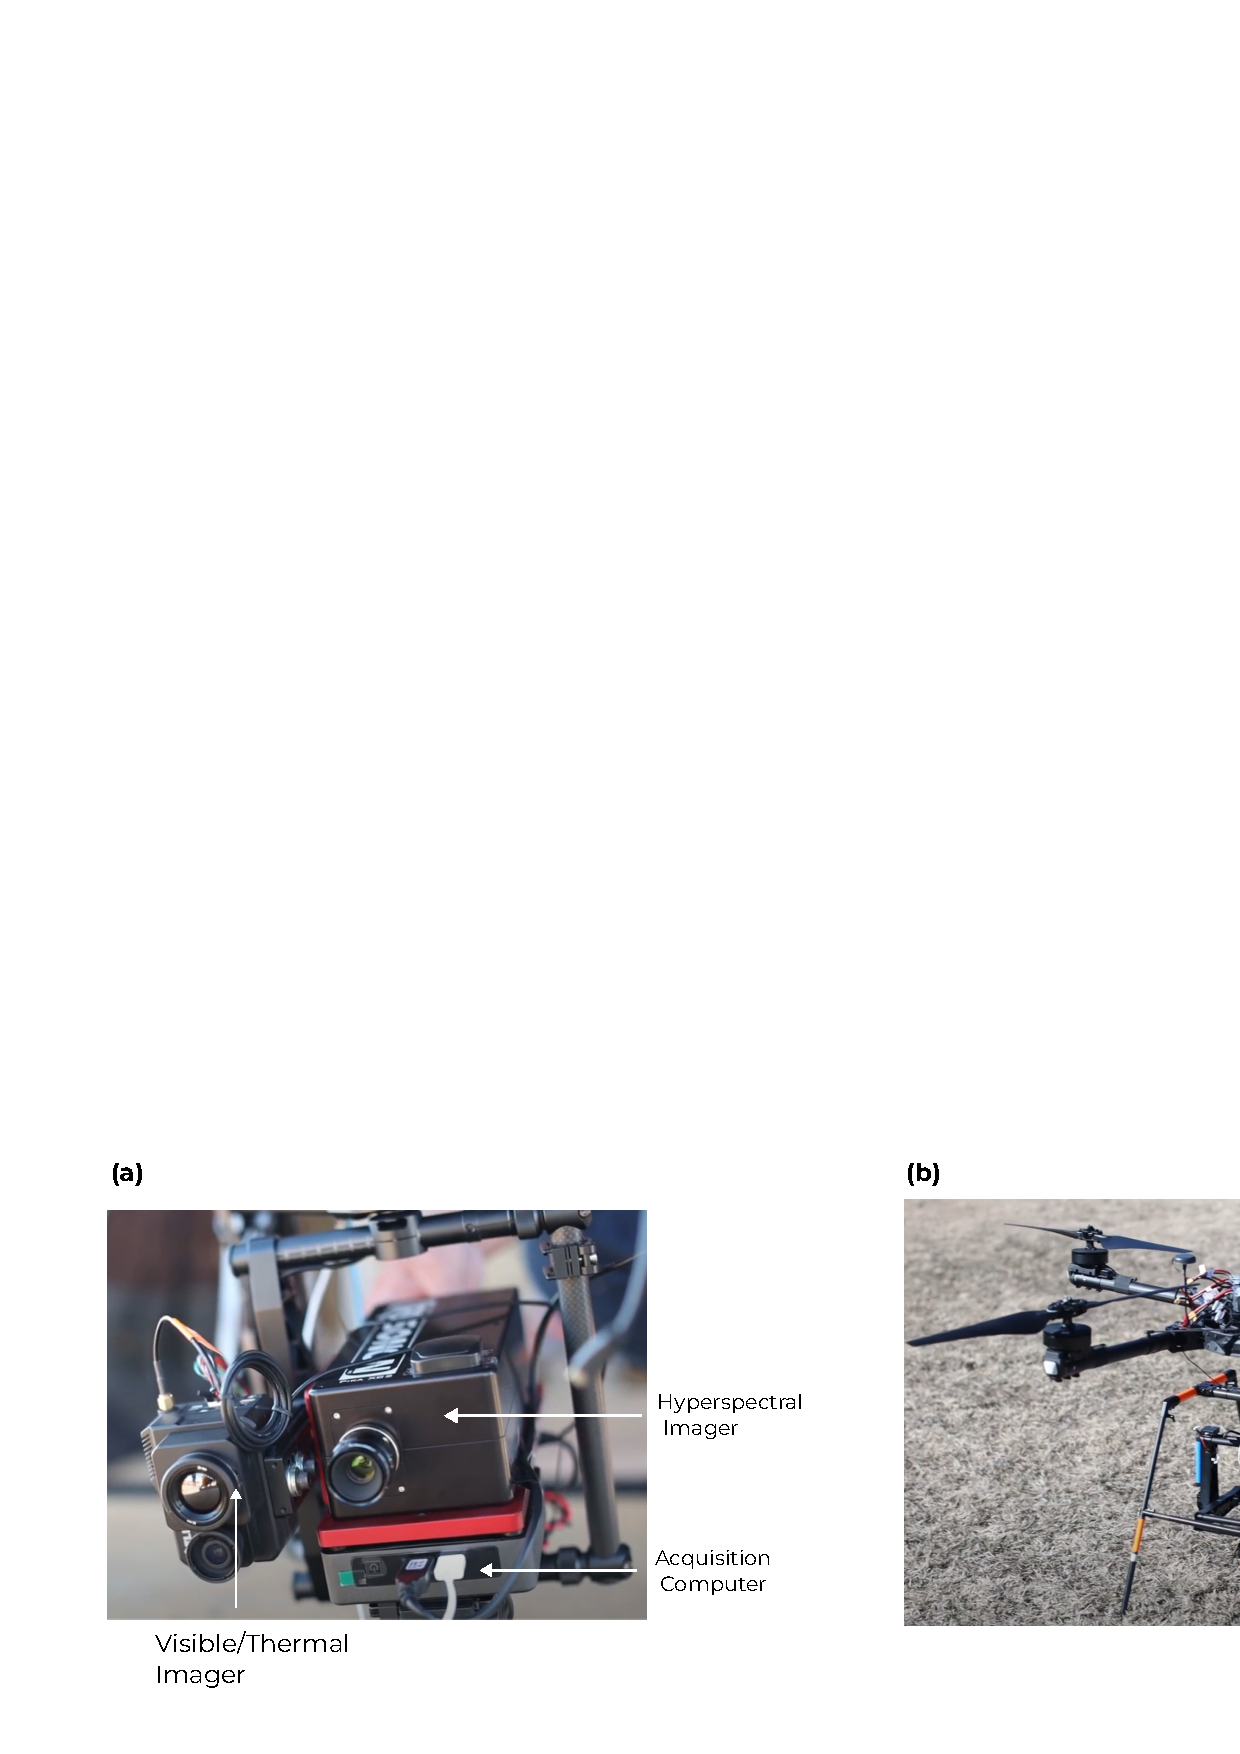
\includegraphics[width=0.85\columnwidth]{robot-team/assets/annotated-drone.pdf}
  \caption{Components of the Autonomous Drone HSI platform.}
  \label{fig:drone-components}
\end{figure}
This spectrometer captures the \textit{downwelling} irradiance spectrum which is necessary to enable conversion from radiance units to the desired reflectance spectra. To this end we present a procedure based on the methods described in \cite{muller-georeferencing, GeorectificationBaumker, GeorectificationMostafa} for the rapid processing and georeferencing of imagery captured by a pushbroom HSI mounted on an autonomous drone. The processing steps are as follows:
\begin{enumerate}
\item Raw imagery are continuously captured by the hyperspectral imager (Radiance) and stored in binary ENVI format.
\item The processing computer reads ENVI files into tensors as they become available.
\item Associated flight data (GPS and IMU) are read.
\item Flight data are interpolated to match the sample times for each scan-line.
\item The HSI is georeferenced to obtain coordinates (lat,lon) for each pixel.
\item The georeferenced HSI is then resampled to a regular grid.
\item The downwelling irradiance spectrum associated with the HSI is read.
\item The downwelling spectrum is interpolated to match the wavelength bins of the HSI
\item The HSI is converted o Reflectance under the assumption of a Lambertian surface (perfectly diffuse).
\item Any desired derived $\lambda$-metrics (NDVI, etc...) are computed.
\item Data products are selected and the result is transferred to the ground station.
\end{enumerate}

\begin{figure}[h]
  \centering
  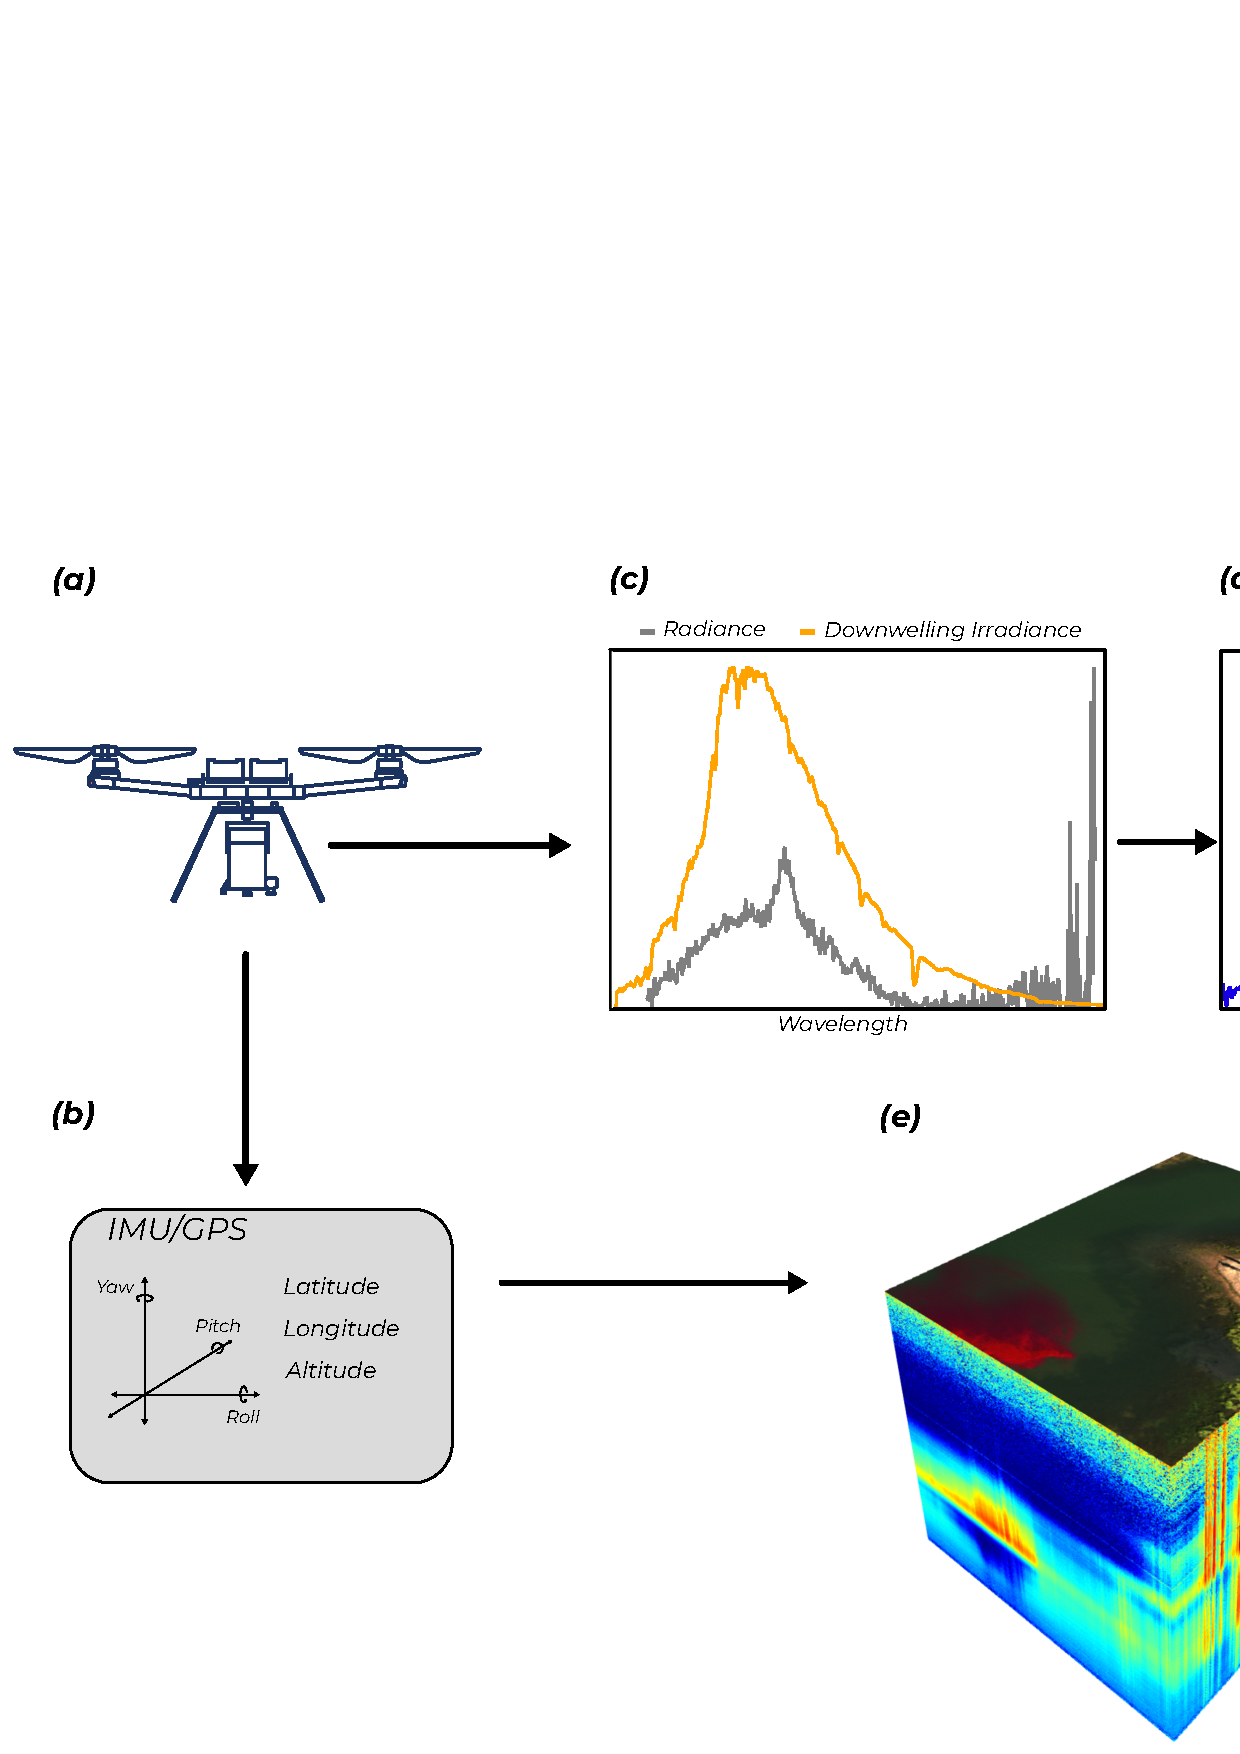
\includegraphics[width=0.85\columnwidth]{robot-team/georectification/pipeline-figure.pdf}
  \caption{Visual representation of the processing pipeline}
  \label{fig:annotated-hsi}
\end{figure}


\subsection{Georeferencing and Resampling}

The hyperspectral imager used on our autonomous drone is different from a typical camera; instead of capturing an image by collecting light onto an array of sensors, our HSI is configured as a pushbroom imager. In this configuration, a single scanline of pixels is captured by the sensor and an image is formed as the drone flies along its route. This poses an interesting challenge for georeferencing as each individual scanline needs to be transformed independently. If the drone's path winds and turns, each subsequent scanline will be stretched and rotated independently based on the relative orientation of the drone to the ground at the time of capture. This sampling geometry as well as the relevant orientation angles are illustrated in Figure \ref{fig:georectification}.

\begin{figure}[h]
  \centering
  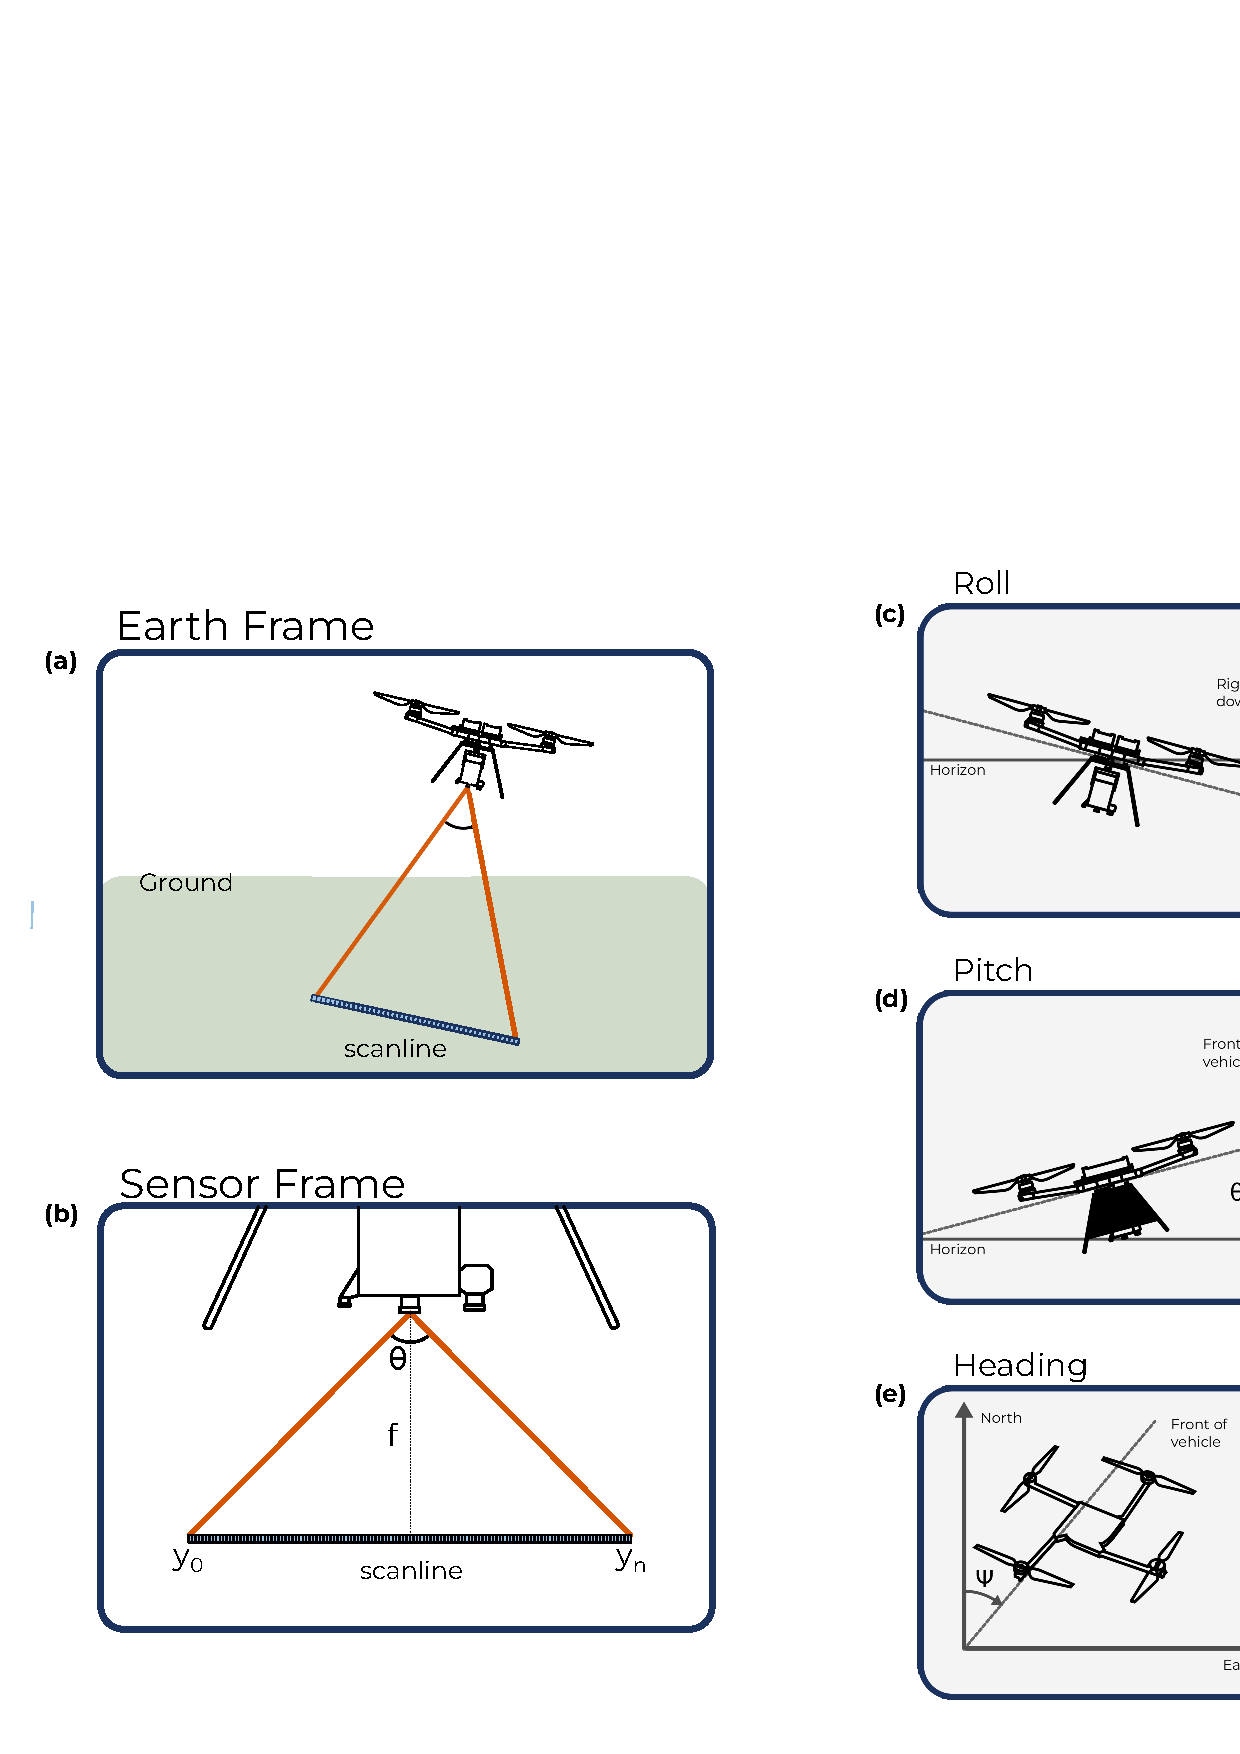
\includegraphics[width=0.85\columnwidth]{robot-team/assets/georectification.pdf}
  \caption{Visual representation of scan-line geometry for the drone based hyperspectral imaging platform.}
  \label{fig:georectification}
\end{figure}

The GPS and IMU on the hyperspectral imager capture the location $(\lambda, \Phi, z)^T$  (longitude, latitude, altitude) of our drone as well it's orientation defined by the angles $\phi$, $\theta$, and  $\psi$ (roll, pitch, and heading) at the time of capture of each scanline. To georeference each pixel, we therefore must transform its position from the frame of the sensor (measured in pixels relative to the HSI) first to the frame of the IMU used to measure the orientation, then to the navigation frame (east, north, up), and finally to the ground frame. Let us define the \textit{sensor} frame so that the scanline falls upon the y axis. As each scanline must be transformed independently, we can assign it an x-coordinate of $0$ pixels. Lastly, if the viewing angle of the HSI is $\theta_{\text{view}}$, then the coordinates of the i\textsuperscript{th} pixel, $\mathbf{r}_i^{\text{sensor}}$, in the sensor frame are defined as in panel (b) of Figure \ref{fig:georectification}, namely
\begin{equation}
  \mathbf{r}_i^{\text{sensor}} = \left(0, y_i, f \right)^T
\end{equation}
where $y_i\in \left\{-\frac{(N-1)}{2},...,\frac{N-1}{2}\right\}$ and $f=\frac{(N-1)/2}{\tan(\theta_{\text{view}}/2)}$ for $N$-total pixels per scanline. To align the sensor frame with the axes of the IMU, we apply a sequence of rotation matrices defined using the measured orientation angles (panels (c), (d), and (e) of Figure \ref{fig:georectification}), which we call
\begin{equation}
  \begin{aligned}
    &R_{\text{sensor}}^{\text{IMU}}(\phi,\theta,\psi) = \\
    &\begin{bmatrix}
    \cos(\psi)\cos(\theta) & \cos(\psi)\sin(\theta)\sin(\phi)-\sin(\psi)\cos(\phi) & \cos(\psi)\sin(\theta)\cos(\phi)+\sin(\psi)\sin(\phi) \\
    \sin(\psi)\cos(\theta) & \sin(\psi)\sin(\theta)\sin(\phi)+\cos(\psi)\cos(\phi) & \sin(\psi)\sin(\theta)\cos(\phi)-\cos(\psi)\sin(\phi) \\
    -\sin(\theta) & \cos(\theta)\sin(\phi) & \cos(\theta)\cos(\phi)
     \end{bmatrix}
  \end{aligned}
\end{equation}

Next, we apply an orthogonal transformation to transform from the IMU frame to the navigation frame of the drone. This is important as the axes of the IMU and the drone itself are not necessarily identical depending on how the IMU is oriented on the HSI. For us, this amounts to
\begin{equation}
  T_{\text{IMU}}^{\text{DRONE}} = \begin{bmatrix}
    0 & 1 & 0 \\
    1 & 0 & 0 \\
    0 & 0 & -1
    \end{bmatrix}
\end{equation}
At this stage, we have now transformed the pixel coordinates into the frame of the drone. Next using the similar triangles defined by the sensor and navigation frames (panels (a) and (b) of Figure \ref{fig:georectification}), we can rescale the coordinates into units of meters by introducing the scale factor
\begin{equation}
  s = \frac{z-z_{\text{ground}}}{f\cos(\theta)}.
\end{equation}
Finally, we translate the coordinates of each pixel using the position of the drone in the chosen coordinate system. As the geometric transformations are scaled to units of meters (by $s$), we apply a coordinate transformation $f$ to obtain the position of the drone with respect to a local coordinate system such as the Universal Transverse Mercator (UTM). Written all together, this takes the form
\begin{equation}
  \mathbf{r}_{i}^{\text{UTM}} =
  f_{\text{geo}}^{\text{UTM}}\begin{bmatrix}
    \lambda \\
    \Phi \\
    z_{\text{drone}}
  \end{bmatrix}_{\text{GPS}}^{\text{geo}} + sT_{\text{IMU}}^{\text{DRONE}}R_{\text{sensor}}^{\text{IMU}}(\theta, \phi, \psi)\begin{bmatrix}
    0 \\
    y_i \\
    f
  \end{bmatrix}^{\text{sensor}}
\end{equation}

For each image, the above transformation can be applied \textit{in parallel} across all scanlines to obtain the ground coordinates $\mathbf{r}_i=(x_i, y_i,z_i)^T$ of each pixel. To aid in further analysis and enable the generation of data products, it is often desirable to resample the georeferenced datacube to a regular grid. To accomplish this rapidly, we can define a bounding box by the extrema of the pixel coordinates. Then, for a desired resolution, say $\Delta x$ in meters, we truncate each pixels coordinates to the nearest $\Delta x$ and then average all pixels that have the same position.


\subsection{Reflectance Conversion}

Once we have georeferenced and resampled the hyperspectral datacube we can use the measured downwelling irradiance spectrum to convert the raw data from radiance to reflectance. This allows us to normalize for the incident light so that spectra captured under variable lighting conditions can be compared. First, the downwelling irraidance spectrum is loaded and interpolated to match the wavelengths of the spectral bins for our HSI. The reflectance at pixel $(i,j)$ and wavelength $\lambda_k)$ is then obtained by
\begin{equation}
  R_{ijk} = \frac{\pi L_{ijk}}{E_k}
\end{equation}
where $L_{ijk}$ denotes the original radiance pixel and $E_k$ denotes the downwelling irradiance at wavelength $\lambda_k$. This conversion makes the assumption that the surface can be treated as \textit{Lambertian}, that is, that the surface is perfectly diffuse and scatters light according to the cosine emission law which when integrated over a half sphere of solid angle introduces the factor of $\pi$.

\begin{figure}[h]
  \centering
  \includegraphics[width=0.85\columnwidth]{robot-team/georectification/hsi-infographic.pdf}
  \caption{Annotated view of a hyperspectral data cube showcasing sampled spectra for a variety of constituents.\label{fig:hsi-infographic}}
  \label{fig:annoted-hsi}
\end{figure}  

Figure \ref{fig:annotated-hsi} illustrates the reflectance spectra for a variety of constituents in a sample hyperspectral data cube. In panel (a) we show a typical downwelling irradiance spectrum. Panels (c)-(f) show a selection of reflectance spectra for open water, a rhodamine dye plume, algae near the shore, and dead grass. Panel (b) is a visual representation of the hyperspectral data cube with reflectance at each wavelength bin along the z axis and a pseudo color image showing the imaging scene on the top.


%%%%%%%%%%%%%%%%%%%%%%%%%%%%%%%%%%%%%%%%%%
\section{Timing Results and Discussion}

The above procedure was implemented in the Julia programming language. Using the package \texttt{BenchmarkTools.jl} the following timings were obtained for each step of the pipeline with results indicating that a hyperspectral datacube of size $1000\times 1600\times 462$ can be georeferenced, resampled, and converted to reflectance in less than 5 seconds at a final spatial resolution of 25 cm.

\begin{table}[!hbt]
  \centering
  \begin{tabular}{ |c|c| }
    \hline
    \textbf{Number of scan lines}	& \textbf{Execution time (s)}\\
    \hline
    371		  &   0.548	\\
    462     &   0.702	\\
    1000    &   1.478  \\
    \hline
  \end{tabular}
  \caption{Loading and georeferencing time as a function of number of scanlines}
  \label{tab:georeference-times}
\end{table}

\begin{figure}[!hbt]
  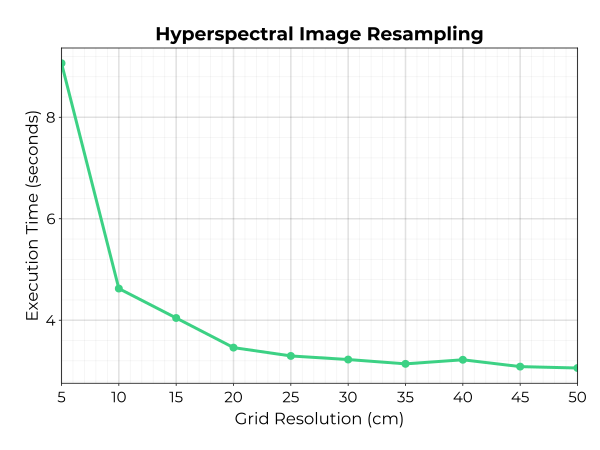
\includegraphics[width=0.85\columnwidth]{robot-team/georectification/regrid-timing.pdf}
  \caption{Timing results (in seconds) for resampling a 1000 scanline HSI as a function of output grid resolution.}
  \label{fig-regridding-timing}
\end{figure}

\begin{table}[h]
  \centering
  \begin{tabular}{ |c|c| }
    \hline
    \textbf{Number of scan lines}	& \textbf{Execution time (s)}\\
    \hline
    371		  &   0.161	\\
    462     &   0.197	\\
    1000    &   0.195  \\
    \hline
  \end{tabular}
  \caption{Loading and georeferencing time as a function of number of scanlines}
  \label{tab:reflectance-times}
\end{table}



%%%%%%%%%%%%%%%%%%%%%%%%%%%%%%%%%%%%%%%%%%



\section{Supervised Regression with Uncertainty Quantification}

The primary modality of our autonomous robotic team is to rapidly characterize the concentrations of chemicals-of-concern in novel aquatic environments. To demonstrate this capability, we performed a sequence of data collections throughout 2020 and 2021 at a ranch in North Texas. Over 3 Tb of hyperspectral imagery were collected across three separate deployments together with ~10,00 in-situ measurements from our autonomous boat. Together these data allow us to train machine learning models whereby direct concentration measurements are utilized to train a family of machine learning models to predict a variety of chemicals of concern. In the rest of this section we present preliminary results demonstrating machine learning models trained to estimate Colored Dissolved Organic Matter (CDOM) concentrations using these datasets.

%% \begin{figure}[!hbt]
%%   \includegraphics[width=0.85\columnwidth]{robot-team/supervised-2/CO/CO_dataMap.png}
%%   \caption{Target distribution of Crude Oil at the ranch in North Texas.}
%%   \label{fig:co-distribution}
%% \end{figure}

\section{Results}
\begin{figure}[!hbt]
  \includegraphics[width=0.75\columnwidth]{robot-team/supervised-2/CDOM/marginalhist.pdf}
  \caption{Stratified train-test split for CDOM}
  \label{fig:train-test-hist}
\end{figure}

Figure \ref{fig:train-test-hist} visualizes a sample distribution of in-situ crude oil concentrations collected by the autonomous boat during our deployments. To build models, each of these records is collocated with associated reflectance spectrum from the HSIs forming a large tabular dataset with spectra as features and concentrations as targets. Additionally, we include a number of derived spectral indices like the Normalized Difference Vegetation Index (NDVI) as well as the drone orientation angles and the relevant solar geometry to provide the model important contextual information about the illumination of the water. The solar zenith, azimuth, and elevation are determined for each pixel using an open source code we implemented in Julia based on a matlab script by Darin Koblick. To train our machine learning models we partition the entire dataset into a train/test split. The bulk of the data is used to train our machine learning models with a representative subsample used as a holdout dataset to evaluate model performance.

\begin{figure}[h]
  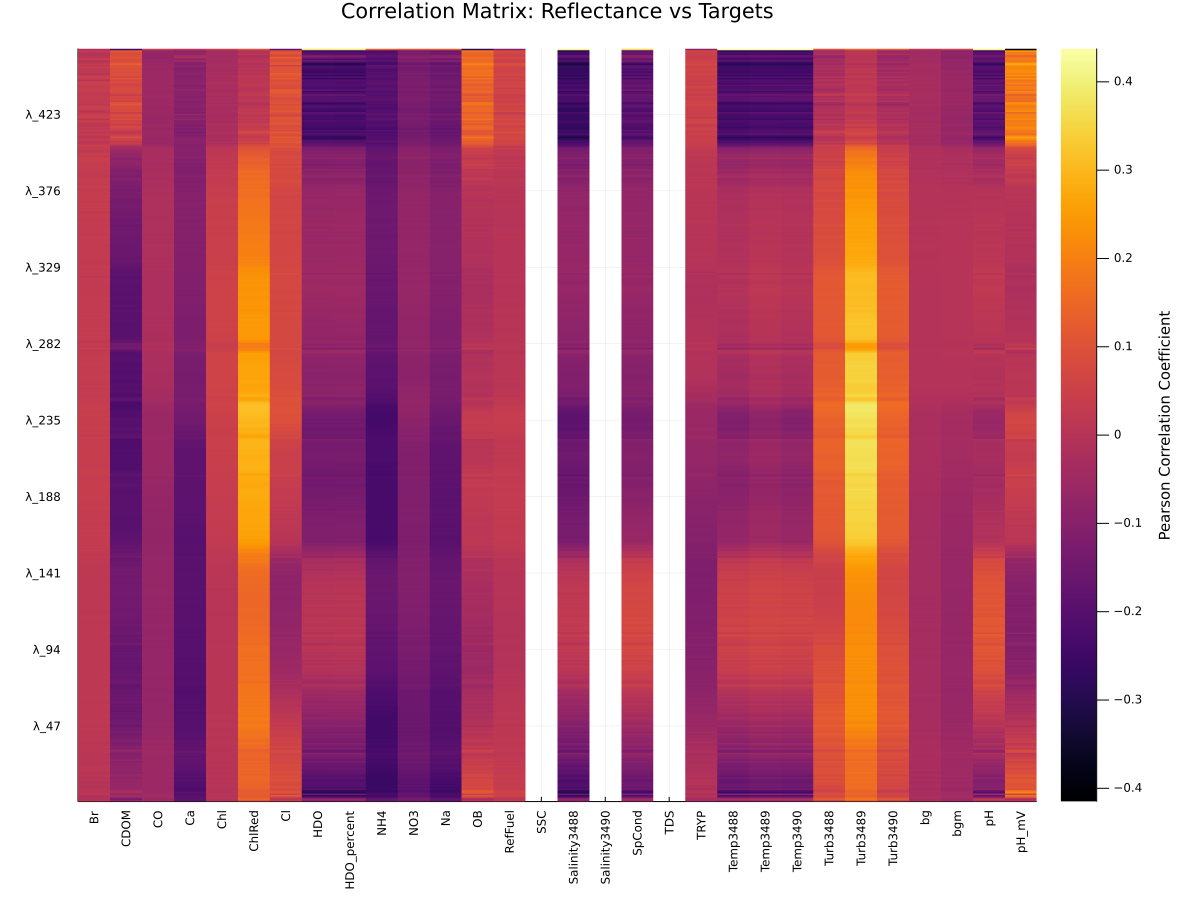
\includegraphics[width=0.85\columnwidth]{robot-team/supervised-2/correlation/reflectance_cor.png}
  \caption{Correlation Matrix for Reflectance measurements versus Target Variables.\label{ref_cor}}
  \label{fig:correlation}
\end{figure}

Figure \ref{fig:correlation} illustrates the correlation matrix between reflectances (as a function of wavelength) and each of the measured targets of the boat. In particular we can see that for CDOM, there is positive correlation between reflectances at long wavelengths  and negative correlation at short wavelengths. This makes sense as crude CDOM tends to absorb broadly in the visible portion of the spectrum and reflects strongly in the infrared leaving water redish-brown. Figure \ref{fig:correlation} also demonstrates how different chemicals of concern can be discerned by absorption features in different wavelength bins.

%% \begin{figure}[h]
%% 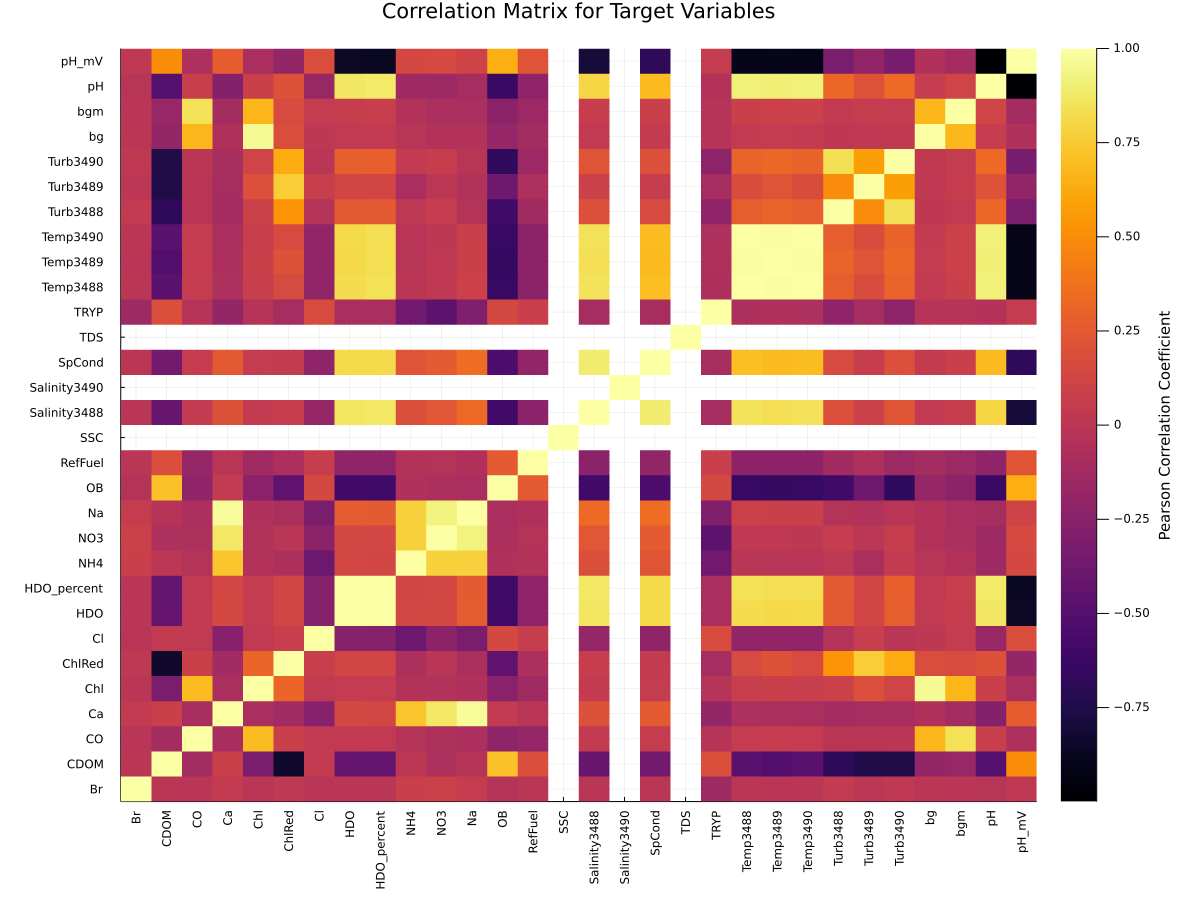
\includegraphics[width=0.85\columnwidth]{robot-team/supervised-2/correlation/target_cor.png}
%% \caption{Correlation Matrix for Target variables measured by the boat.\label{target_cor}}
%% \end{figure}

%% \begin{figure}[h]
%% 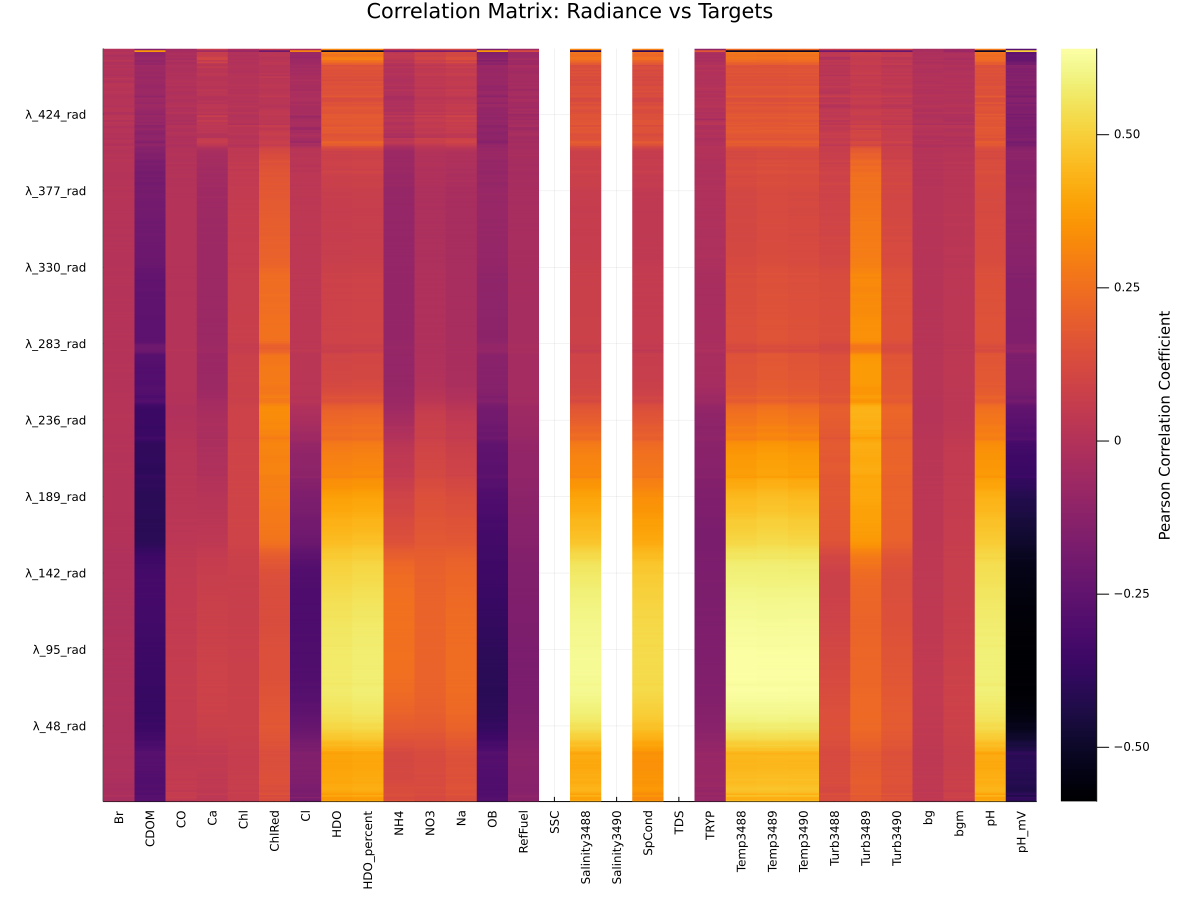
\includegraphics[width=0.85\columnwidth]{robot-team/supervised-2/correlation/radiance_cor.png}
%% \caption{Correlation Matrix for Radiance measurements versus Target Variables.\label{rad_cor}}
%% \end{figure}

%% \begin{figure}[h]
%% 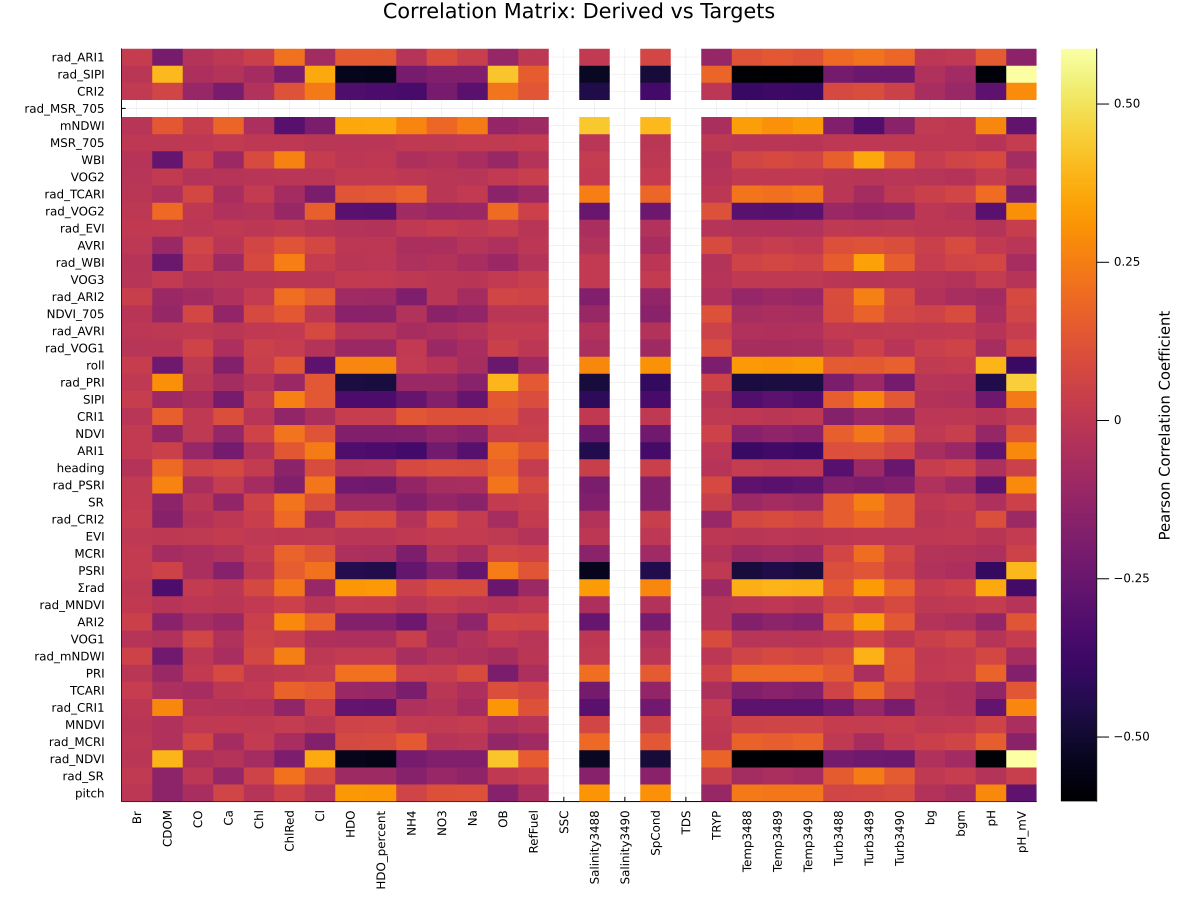
\includegraphics[width=0.85\columnwidth]{robot-team/supervised-2/correlation/derived_cor.png}
%% \caption{Correlation Matrix for derived measurements versus Target Variables.\label{derived_cor}}
%% \end{figure}

\subsubsection{Results So Far}

For our machine learning approach, we've employed a an ensembling strategy called \textit{model stacking} (also known as a \textit{super-learner}) \cite{ModelStacking}. Rather than arbitrarily choosing a single model such as a neural network or decision tree, we form a \textit{stack} of many models including linear regression, neural networks, decision trees, gaussian process regression, random forest, and boosted trees (XGBoost and EvoTrees). A discriminator model (i.e. the super learner) is then trained on the output of each base model in order to effectively combine the results to generate a robust prediction \cite{ModelStacking}. To prevent the super learner from simply siding with the best \textit{average} model, the training dataset is carefully partitioned into a set of $N$ cross validation folds. For each fold, every base model is trained on the $N-1$ fold complements and produces a set of out-of-bag predictions for the chosen fold. These predictions are the stitched together and used to train the super learner. Once the super learner is trained, the original base models are retrained on the entire dataset with the resulting stack of base learners plus discriminator forming the final predictive model.

\begin{figure}[!hbt]
  \begin{subfigure}{0.5\textwidth}
    \centering
    \includegraphics[width=0.95\linewidth]{robot-team/supervised-2/CDOM/scatterplt__stack.pdf}
  \end{subfigure}
  \begin{subfigure}{0.5\textwidth}
    \centering
    \includegraphics[width=0.95\linewidth]{robot-team/supervised-2/CDOM/qq__stack.pdf}
  \end{subfigure}
  \caption{(\textbf{a}) Scatterplot for the trained CDOM super-learner model. (\textbf{b}) Quantile-Quantile plot for the same fit.}
  \label{fig:CDOM_fitresult}
\end{figure}

Figure \ref{fig:CDOM_fitresult} illustrates the quality of the resulting super-learner fit. The combined dataset is largely tri-modal with three large peaks. Consequently, the model performs best near these values with the worst performance occurring at low concentrations with sparse samples.

A number of the models involved in our super-learner employ a decision-tree based learner. For these base learners we can evaluate the relative importance of each input feature to the predictions of the model. These feature importances are ranked in Figure \ref{fig:CDOM-fi}.
\begin{figure}[!hbt]
    \includegraphics[width=0.85\columnwidth]{robot-team/supervised-2/CDOM/importance_ranking__vanilla.pdf}
    \caption{Ranked feature importance for CDOM.}
    \label{fig:CDOM-fi}
\end{figure}
This feature ranking reveals that wavelengths in key portions of the visible spectrum have the largest impact on model predictions. Similarly, the Solar Altitude and Drone pitch/heading are ranked highly due to the important impact of the solar illumination and viewing geometry on the captured spectra. Using these models, we can rapidly generate wide area maps that estimate concentrations at all HSI pixel location. Sample maps for both CDOM and Crude Oil are shown in Figure \ref{fig:lary-maps}.

\begin{figure}[!hbt]
  \includegraphics[width=0.9\columnwidth]{robot-team/assets/CrudeOil-CDOM-Maps.png}
  \caption{Maps of Crude Oil and CDOM generated using the trained super-learner models.}
  \label{fig:lary-maps}
\end{figure}

Figure \ref{fig:lary-maps} generates precisely how this Robotic Team can be used to generate actionable environmental insights. Both of these chemicals-of-concern are observed to collect in a region of the pond that is largely isolated with little flow. However, because we were able to acquire samples from this region we are also able to identify accumulation occurring near the shores.


\subsubsection{Next Steps}

The next steps for this supervised approach are to incorporate conformal prediction into the super-learner model pipeline. By partitioning a third hold out dataset, we can simultaneously estimate the concentrations using our trained super learner \textit{and} obtain reasonable uncertainty bounds for these predictions. With the ability to generate uncertainty estimates together with our model predictions, we can develop \textit{smart} data collection strategies to enable the robotic boat to collect additional samples optimized to decrease model uncertainty and not waste time re-treading portions of the pond where the model is already highly confident.

\section{Methods for Unsupervised Classification of Hyperspectral Scenes in Novel Environments}

A second modality for the robotic team is to utilize unsupervised machine learning strategies to identify key constituents for which we \textit{do not} have reference sensors. Many common approaches like endmember mixing models treat measured reflectance spectra as a linear combination of representative source spectra whose coefficients indicate a relative abundance within a pixel. By utilizing the Self Organizing Map and Generative Topographic Map codes I've developed, we can identify key endmembers present in the scene for which the autonomous boat is not equipped to directly measure. Further, by examining the learned weights of each class and their distribution throughout the scene, we can attempt to assign individual classes to known chemical signatures.

\subsubsection{Unsupervised Classification}
\begin{figure}[h]
  \includegraphics[width=\columnwidth]{robot-team/unsupervised/clustering.png}
  \caption{Unsupervised clustering of hyper-spectral image data using the K-means algorithm.\label{clustering}}
\end{figure}




